
%%%%%%%%%%%%%%%%%%%%%%%%%%%%%%%%%%%%%%%%%%%%%%%%%%%%%%%%%%%%%%%%%%%%
\section{Installation, Integration and Commissioning}
\label{sec:fdsp-daq-install}

%%%%%%%%%%%%%%%%%%%%%%%%%%%%%%%%%%%%
\subsection{Installation}
\label{sec:fdsp-daq-install-transport}

The majority of \dword{daq} components will be installed in a dedicated and partitioned area of the CUC (`counting room') as shown in Figure~\ref{fig:daq-install-controlroom}, starting as soon as the consortium has beneficial occupancy of this space. Fiber will be run from both the detectors' \dwords{wib} to the \dword{daq}, and from the \dword{daq} to the surface, installed by the CF group. This starting point is currently projected to be eighteen months before \dwords{apa} can be installed in cryostats of the first module, allowing time for final component acceptance testing in the underground environment, and for the \dword{daq} to be ready to be used for detector testing and commissioning. Some \dword{daq} components (event builder, storage cluster and WAN routers, plus any post-event-builder processing) will be installed above ground.

\SI{500}{kVA} of power and cooling will be available to run the computers in the counting room. 12 standard \SI{19}{in} server racks (of up to 58U height) per module have initially been allocated for each detector module, with two more each for facilities and CISC. An optimised layout, including the necessary space for hardware installation and maintenance, plus on-site spares, will be developed once the final \dword{daq} design is known. The racks will be water cooled with local air-to-water heat exchangers. To allow expanded headroom for initial testing, development, and commissioning throughput, the full complement of rack infrastructure and network equipment will be installed from the start, even though only the first two modules will need to use it.

\begin{dunefigure}[CUC Control Room Layout]{fig:daq-install-controlroom}
  {Floor plan for the \dword{daq} and control room space in the CUC.  The `\dword{daq}
    Room' has space for at least 52 racks of servers and routers.
    Fiber from the \dwords{wib} in the detector caverns will enter in the upper
    right of this room, terminate in a breakout panel, and be
    distributed to the \dwords{rce} in these racks, then to \dword{felix} servers (also
    in this room) as outlined in
    Figure~\ref{fig:daq-readout-buffering-baseline}.  Fibers to the
    surface will enter this room from the lower left.}
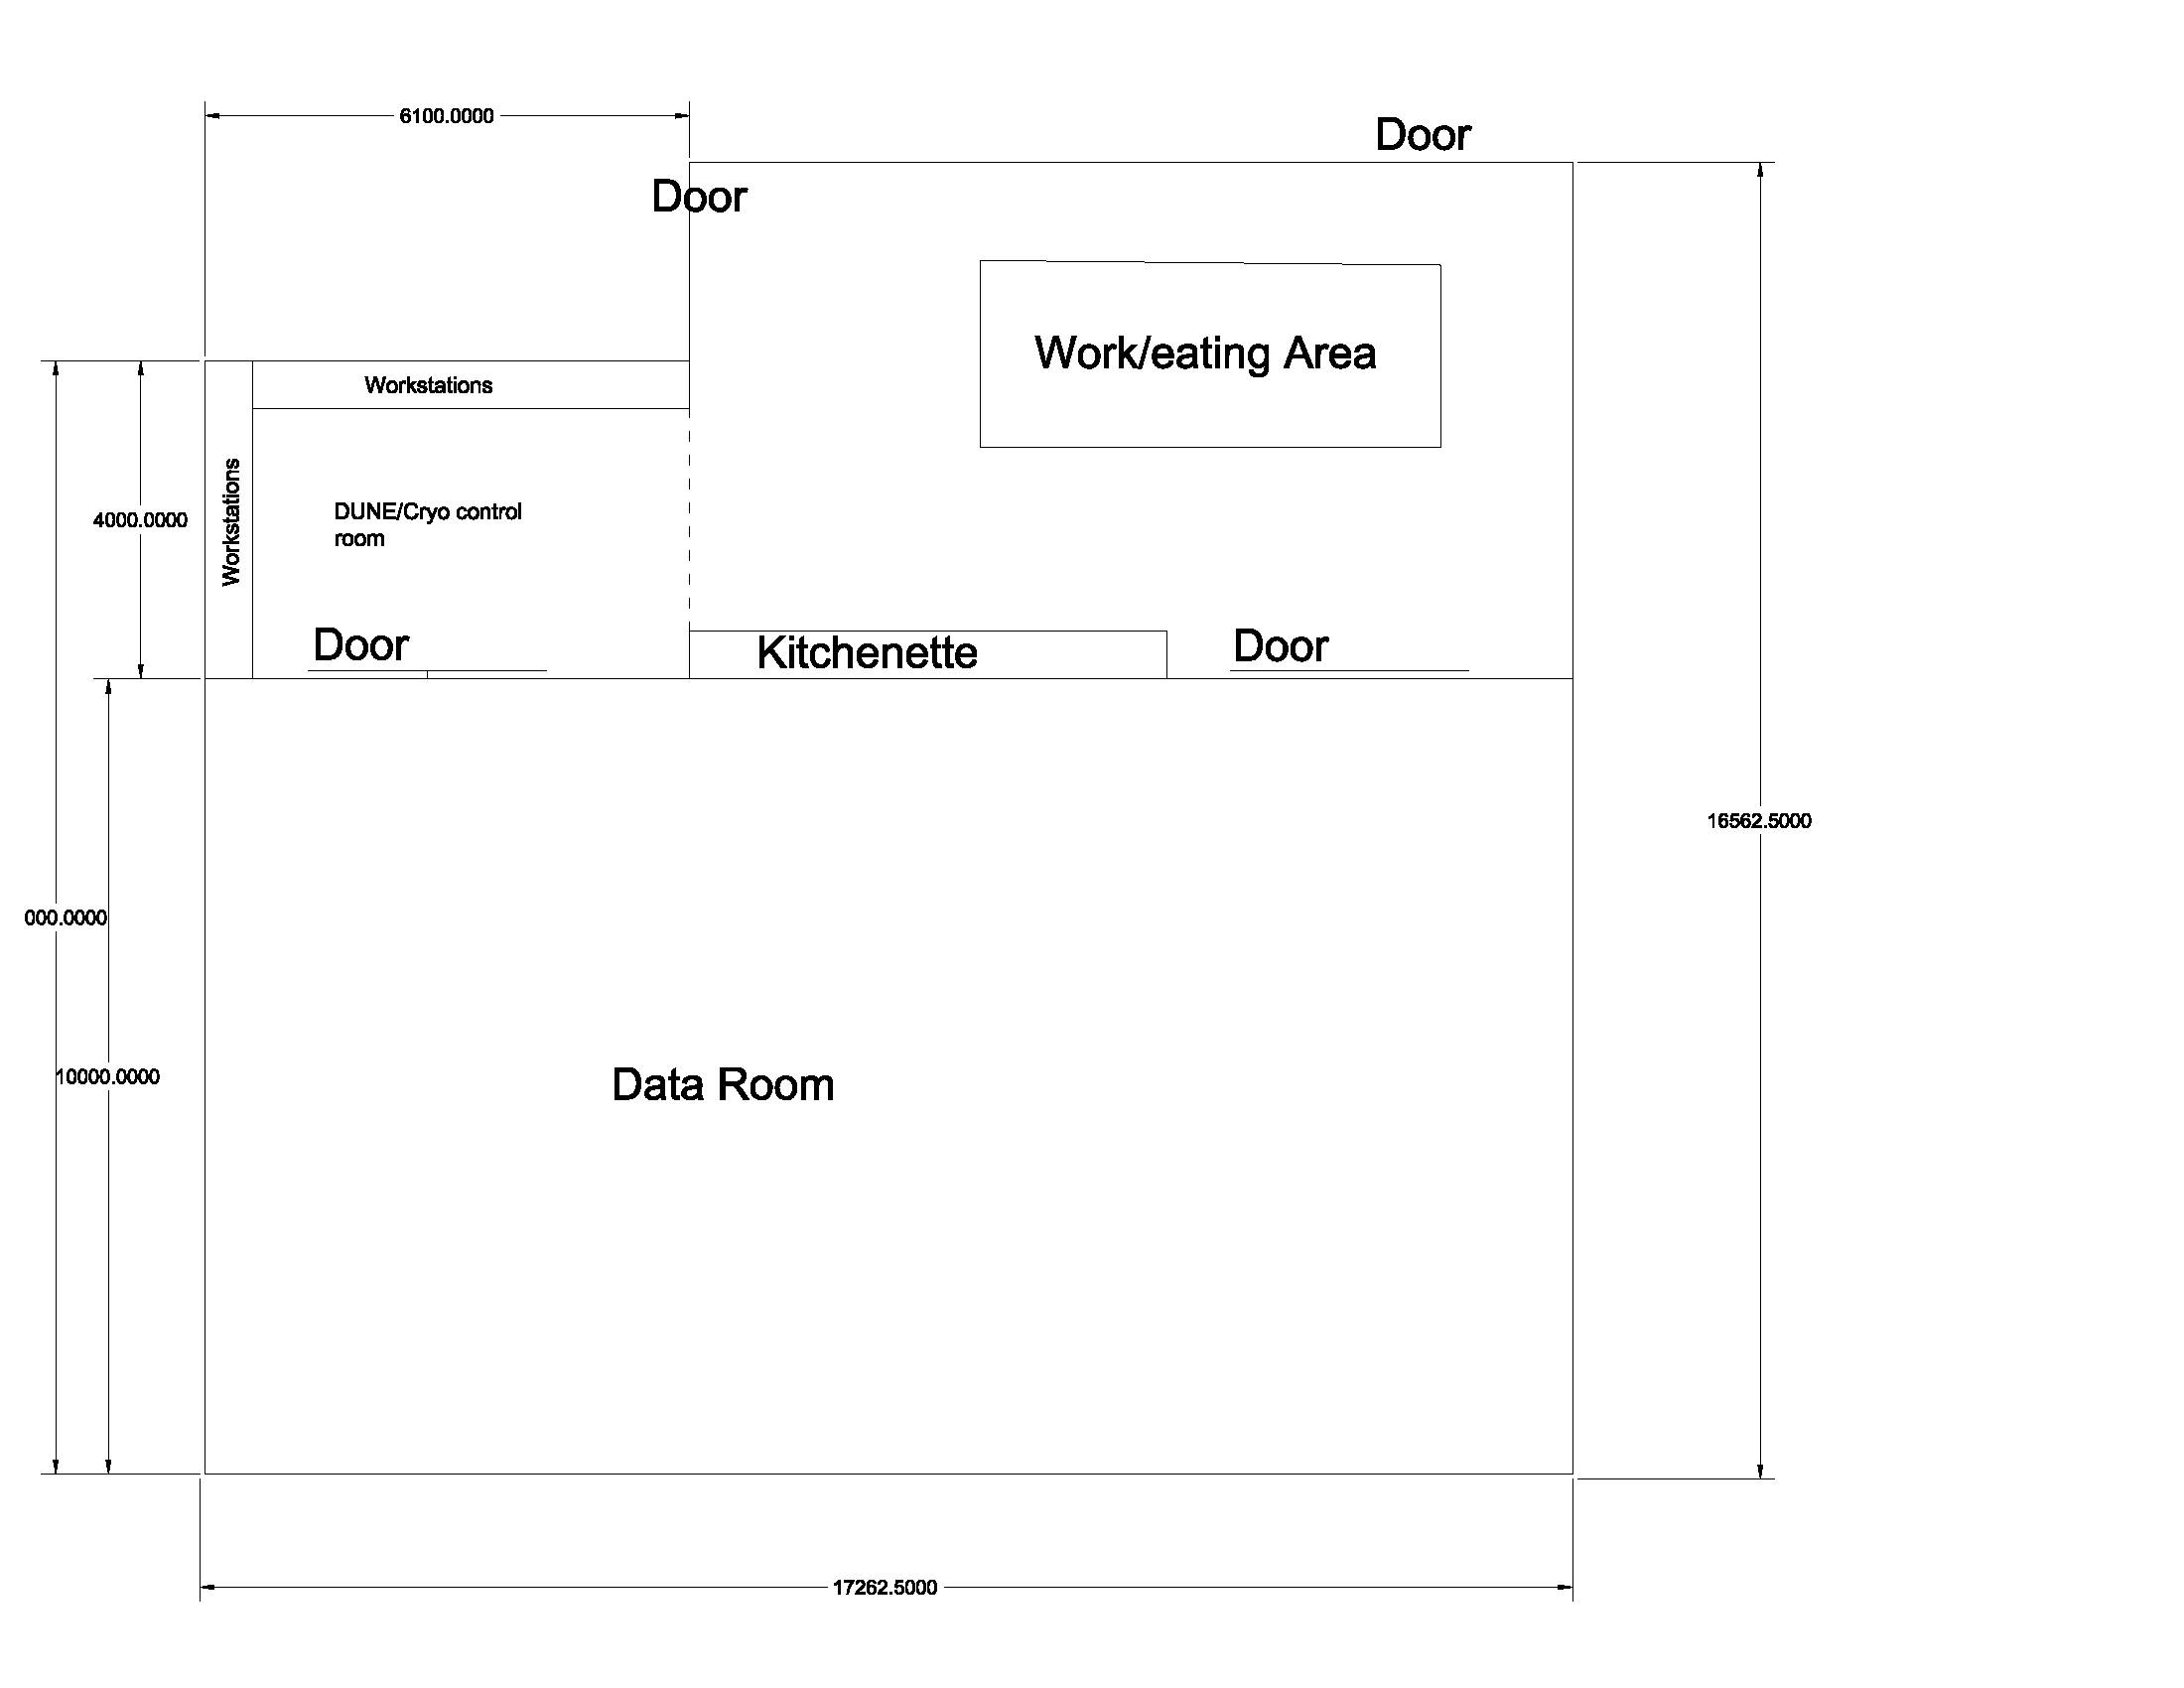
\includegraphics[width=0.8\textwidth]{ControlRoom-v2.png}
\end{dunefigure}

The counting room will be similar to a server room at a university or national lab in terms of need for cleanliness, ventilation, fire protection, drop flooring, and access control. Networking infrastructure and fiber breakout will take up some of the rack space, but not very much of the power budget. Power to individual machines and crates will need to be controlled remotely via power distribution units, as a goal is to minimize \dword{daq} workers' presence underground if there is work which can be done from the surface or remotely.  Some UPS capacity will be needed to allow for an orderly shutdown of computers, but only networking equipment will need longer duration backup power, to enable remote recovery from short-term power failures.  

%%%%%%%%%%%%%%%%%%%%%%%%%%%%%%%%%%%%
\subsection{Integration with detector electronics}
\label{sec:fdsp-daq-install-transport}

Basic technical integration with detector electronics will take place before installation, during a number of integration exercises in the preceding years. We anticipate that the consortium will supply and support small-scale instances of the \dword{daq} system for testing of readout hardware at the production sites, based on prototype or pre-production hardware. Full-scale \dword{daq} testing will have been completed with artificial data sources during internal integration. The work to be done during installation is therefore essentially channel-by-channel verification of the final system as it is installed, on a schedule allowing for any rectifying work to be carried out on the detector immediately (i.e. the \dword{daq} must gather and present data in effectively real time). This implies the presence of a minimal but sufficient functional \dword{daq} system before detector installation commences, along with the timing and fast control system, and the capability to permanently record data for offline analysis. However, it does not require triggering, or substantial event building or data transfer capacity. The \dword{daq} installation schedule is essentially driven by this requirement.

In addition, the data pipeline from event builder, via the storage buffer and WAN, to the offline computing facilities, must be developed and tested. We anticipate this work largely happening at FNAL in parallel with detector installation, and the full-scale instances of these components being installed at SURF in preparation for start of data-taking.

%%%%%%%%%%%%%%%%%%%%%%%%%%%%%%%%%%%
\subsection{Commissioning}
\label{sec:fdsp-daq-commissioning}

System commissioning for \dword{daq} comprises the following steps:

\begin{itemize}
	\item Integration with detector subsystems of successive modules
	\item Final integration and functional testing of all \dword{daq} components
	\item Establishment of the necessary tools and procedures to achieve high-efficiency operation
	\item Selection, optimisation and testing of trigger criteria
	\item Ongoing and continuous self-test of the system to identify actual or imminent failures, and to assess performance
\end{itemize}

Each of these steps will have been carried out at the integration test stands before being used on the final system. The final steps are to some extent continuous activities over the experiment lifetime, but which require knowledge of realistic detector working conditions before final validation of the system can take place. We anticipate that these steps will be carried out during the cryostat filling period, and form the major focus of the \dword{daq} consortium effort during this time.
